\begin{fullwidth}
\chapter{A modelling oriented primer on cholera}
\end{fullwidth}
Cholera is an acute intestinal infection causing severe diarrhea that may lead to dehydration, and sometimes death. While the global burden of cholera is difficult to estimate as the majority of cases are not reported, it is estimated that 3 million cases and 95'000 deaths occurs every year in endemic areas (around 50 countries), with millions more at risk\cite[-1\baselineskip]{Ali:UpdatedGlobalBurden:2015}. Despite its household name, cholera belongs to the neglected tropical diseases group as our understanding of many important aspects of cholera clinical course and transmission is limited.
A political will to eliminate this ancient disease has recently arisen. The World Health Organization (WHO) initiated the Global Task Force for Cholera Control (GTFCC), who provides a concrete path towards the elimination of cholera by 2030\footnote[][-3\baselineskip]{Elimination being defined as a 90\% reduction of cholera deaths/year, see \url{gtfcc.org} for more information.}. The general consensus is that to reach this goal in endemic countries, there must be substantial long-term improvements in safe water distribution systems, adequate sanitation and accessible hygiene education.  Moreover, in the event of a cholera outbreak, timely interventions such as vaccination campaigns are crucial to limit the spread of the disease, and proper medical treatment reduce the toll of the disease on communities. %With limited resources, public health officials face a number of challenging decisions, and a data driven decision support to guide the rational deployment of cholera control strategies is needed. Furthermore, on the road toward elimination, the need to setup context-specific tailored approaches appears. 
%The poorest of the poor
%most infected individuals are asymptomatic, i.e., they do not present symptoms, while other experience mild or severe symptoms.  %Since their mobility is not hindered, they become a vector of the infection. If not properly treated, cholera can kill children and adults within hours. 


\vspace{.7cm}
\section{History and epidemiology}
\begin{marginfigure}[-4\baselineskip]
%\centering
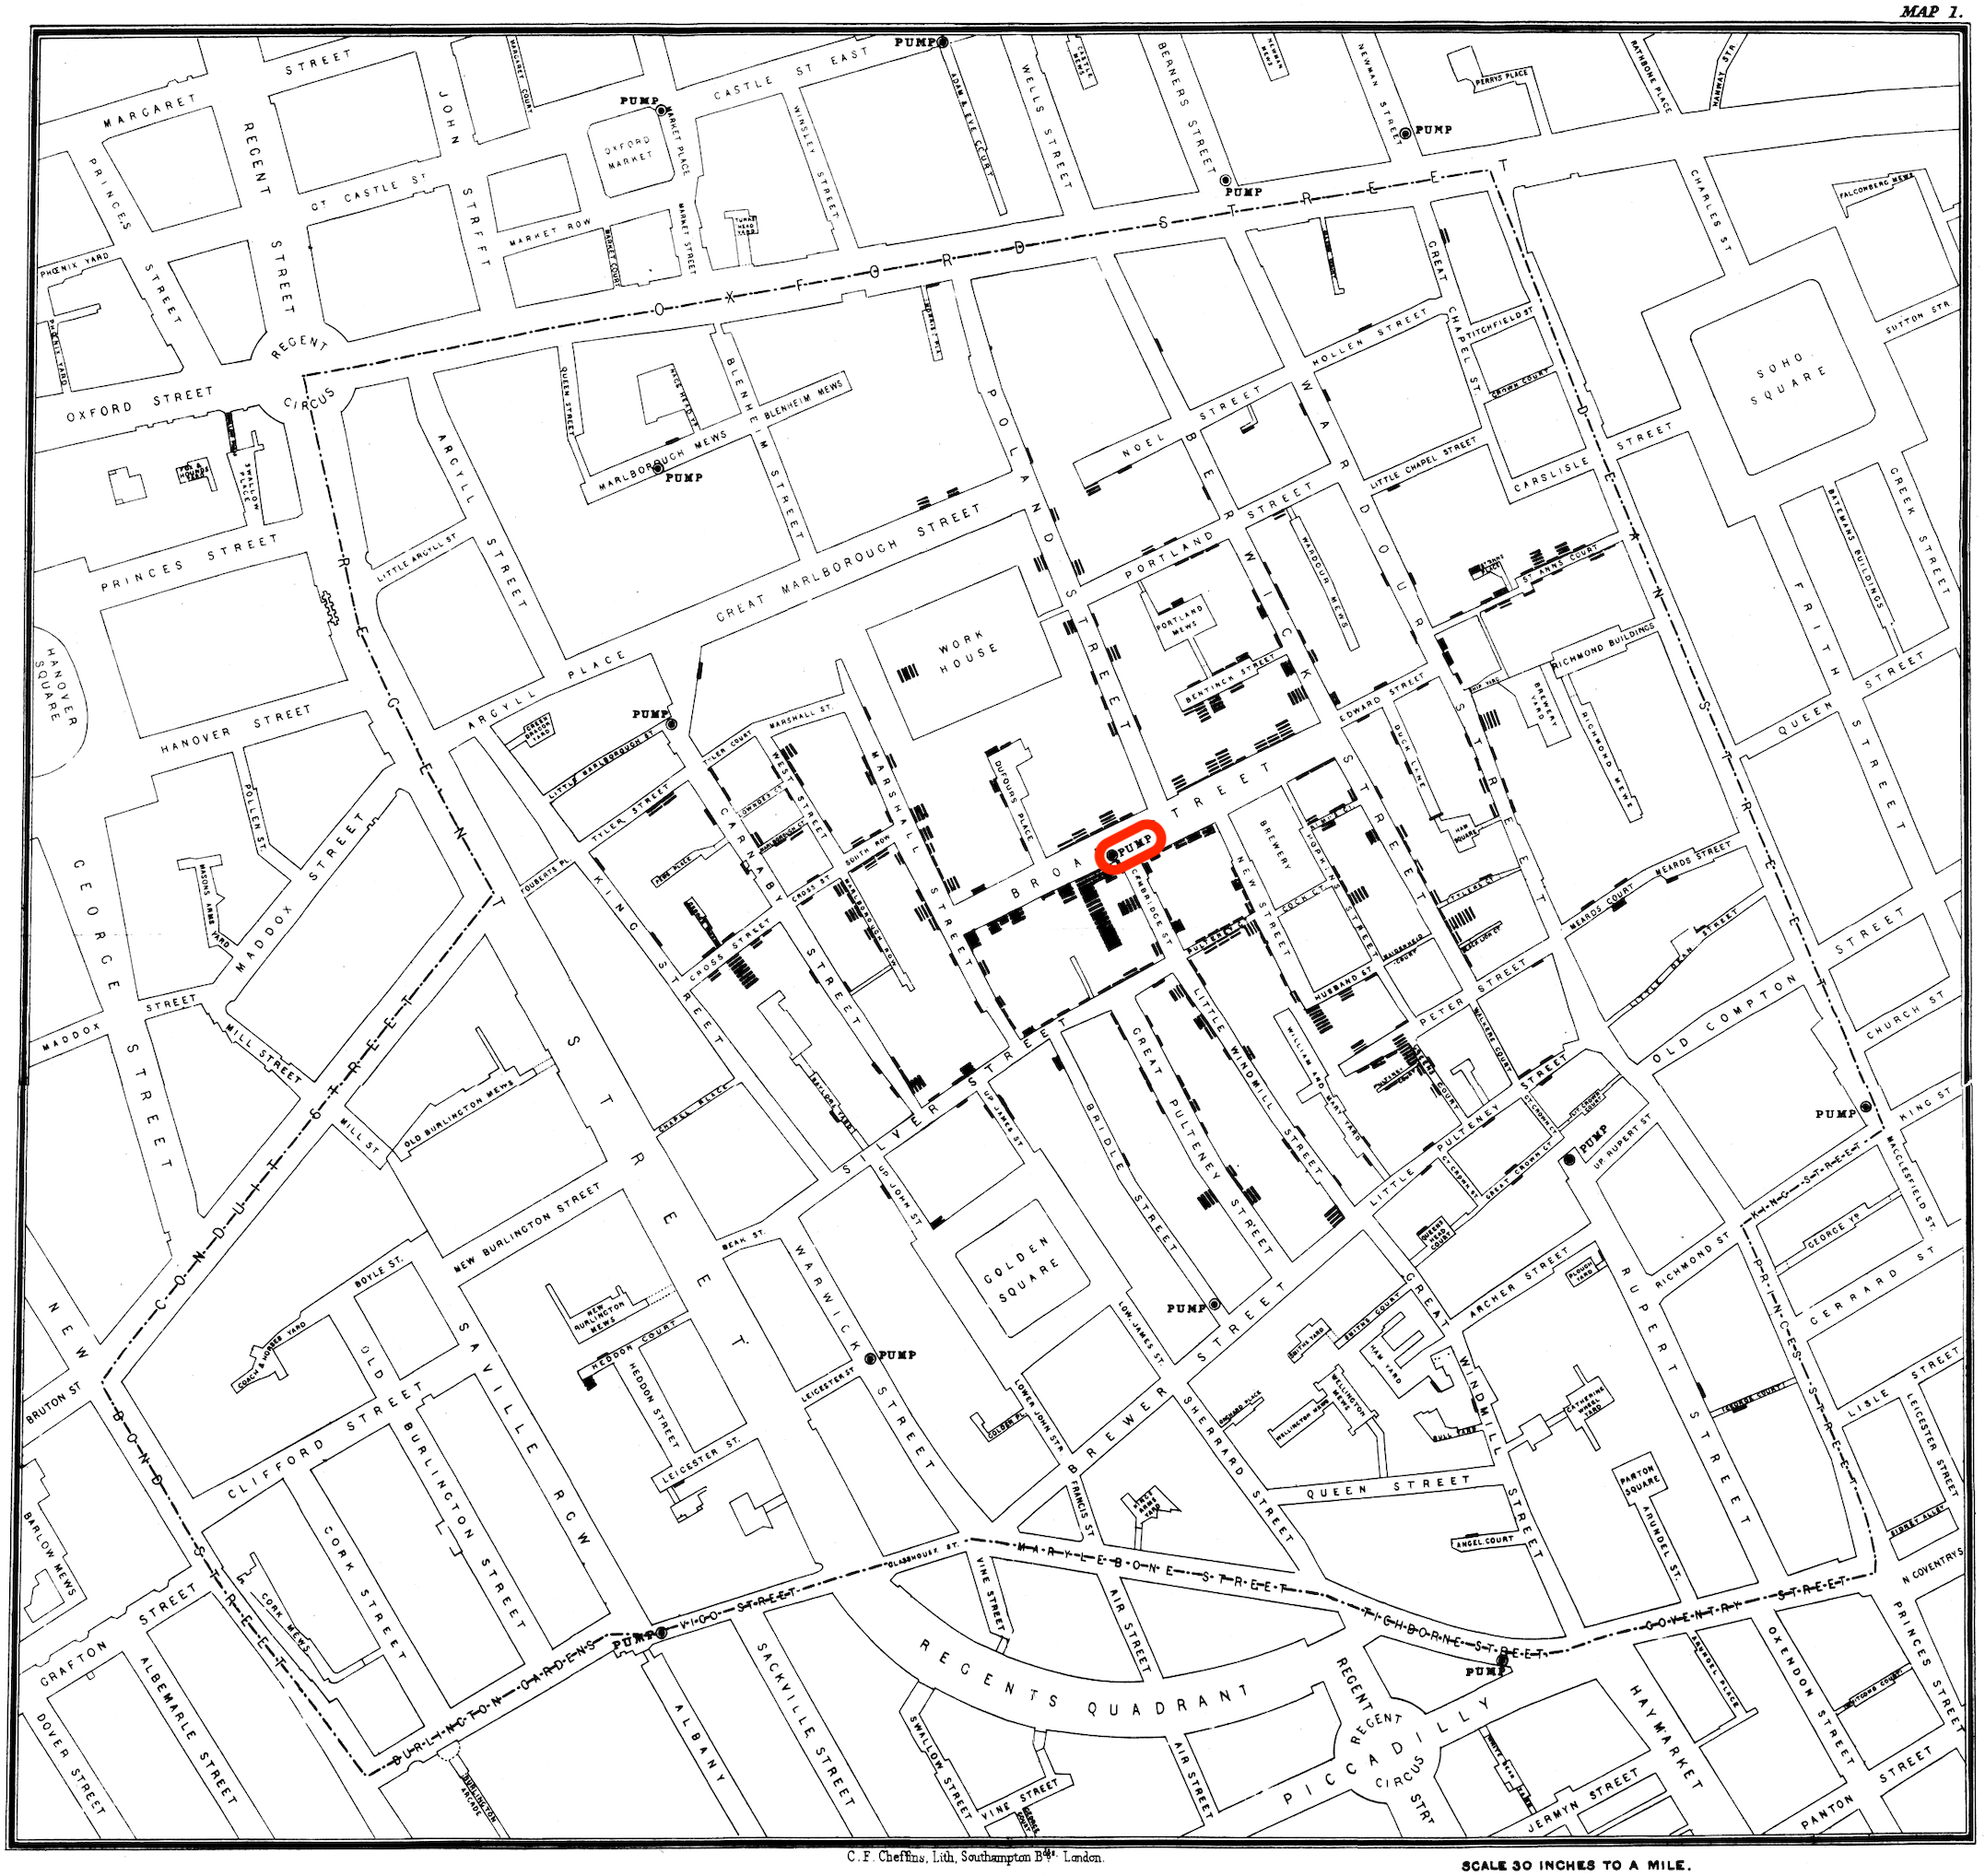
\includegraphics[width=\textwidth]{fig/snow-cholera-map_edit}
\margincaption[John Snow map of cluster cholera cases in London, 1854]{Original map by John Snow. Stacked rectangles represent cholera cases of the 1854 Broad Street outbreak. The work of John Snow conviced the authorities to close the water pump (circled in red), leading to a decrease in Mortality. Lithography by Charles Cheffins, in \fullcite[p. 54]{Snow:ModeCommunicationCholera:1855}.}\label{johnsnow}
\end{marginfigure}
Humanity and cholera share a long history, with supposed mentions as early the 5th century \textsc{bce}. The disease became more widely know in the modern era. From 1817 to 1923, six successive pandemics -- all originated in the delta of the Ganges river, but taking different paths accross the world -- occured. Cholera spread around the world owning to the the nascent mobility, leaving 10s of millions dead accross countries and continents.  Scientific developments sped up during the third cholera pandemic (1846-60). In 1854, a cholera outbreak in Broad Street (Soho, London) was studied by physician John Snow and lead to an impressive early work in investigative epidemiology and public health. Analyzing the contamination pattern among residents, Snow postulated that cholera spread through water contaminated by an infectious agent, instead of foul air\sidenote[][-3\baselineskip]{At the time, the accepted mode of contamination for cholera and many other disease was through miasma, \textit{bad air} contaminated by organic matter. Chasing odor justified urban plannings along streets and river banks in Paris and London. But also in Lausanne, where rivers Flon and Louve where covered in 1832 in response to a cholera outbreak. Cholera is the name of a savoury dish from Valais is a testimony of the strong impression cholera left on the Swiss.}.  Simultaneously, Italian microbiologist Filippo Pacini isolated the bacterium in Florence\cite{Pacini:OsservazioniMicroscopicheDeduzioni:1854}. Thirty years after Pacini, German scientist Robert Koch independently rediscovered the cholera pathogens after investigation in Egypt and India and first posited its causative relationship with the disease. Finally a hundred year later, Indian researcher Sambhu Nath De discovered the cholera toxin in 1959\cite{De:ExperimentalStudyAction:1951}.

Throughout the seventh pandemic from 1961 onwards, cholera spread in several waves, through Asia in the 1960s, reachin Africa and the Middle East in the 1970s and the Americas in 1991\cite{Mutreja:EvidenceSeveralWaves:2011}. Improvement in sanitation and hygiene spared higher income country from disease, and cholera became a burden of the poorest of the Global South. Series of outbreaks (\eg Zimbabwe 2008, Haïti 2010, Yemen 2016), continuous transmission in endemic countries and millions at risks keeps this ancient disease a ongoing public health issue.

The span of this thesis was marked by a cholera outbreak in Yemen (2016--2021) -- an humanitarian crisis with 2.5M suspected cases and nearly 4'000 deaths -- an outbreak in Zimbabwe and flare up in Algeria in addition to seasonal outbreaks and endemic cholera transmission in the Asia and sub-saharian Africa.  But also by the last confirmed cases of cholera in Haiti in 2019.

While the number of cholera cases doubled from 2018 to 2019 to nearly a million, reported cholera death decreased to less than 2'000 in 2019, with Africa reporting lowest number since the 2000s. Haiti reported its last confirmed cholera cases in january 2019, bringing hope to cholera elimination from its last foothold in the Americas. Effort towards improvement of sanitary conditions and reactive vaccinations (24M doses of cholera vaccines were distribued in 2019) hope to bring these number down\footnote{see \fullcite{WHO:Cholera2019:2020} and previous \textit{Weekly Epidemiological Records} about cholera.}. 

In the following is highlighted some relevant aspects about cholera transmission, while leaving some biological and medical features of cholera outside the scope of this thesis.


\section{Epidemiology} 
\begin{marginfigure}[6\baselineskip]
\centering
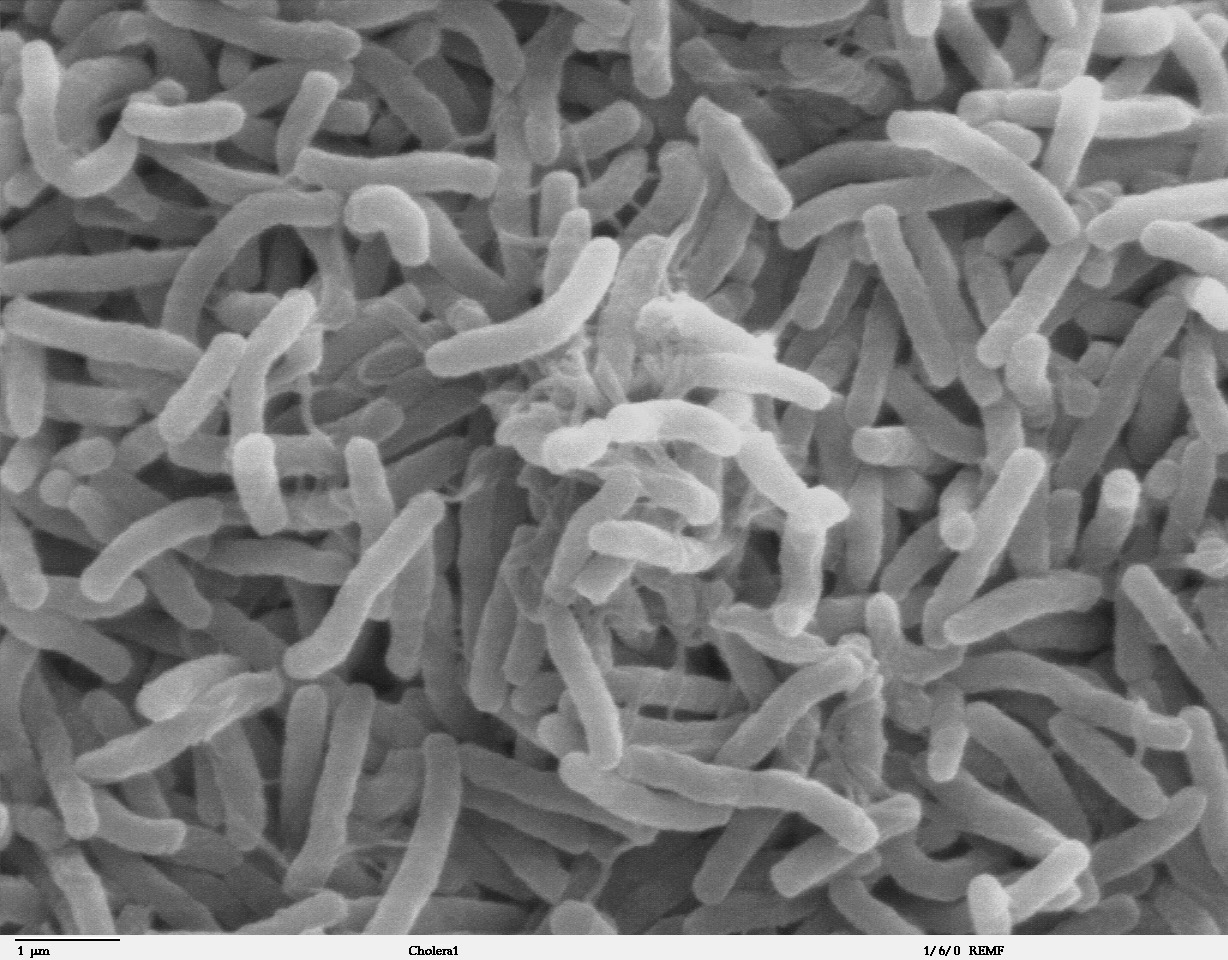
\includegraphics{fig/vibrio}
\margincaption[Vibrio cholerae bacteria]{Scanning electron microscope image of \textit{Vibrio cholerae},  a gram-negative rod-shaped bacteria (Public domain image by Ronald Taylor, Tom Kirn, Louisa Howard).}
\label{fig:bacteria}
\end{marginfigure}
\paragraph{Pathogen} Cholera is an infection caused by a waterborne bacteria: the \emph{Vibrio cholerae}. While many serogoups of \emph{V. cholerae} can secrete the cholera toxin reponsible for massive watery diarrhea, only serogoups O139 and O1 are responsible for disease epidemics. O1 is causing most recent epidemics, and is divided in two biotypes: Classical O1 and El Tor, which are both divided into three serotypes: Ogawa, Inaba and the rare Hikojima\cite{Kaper:Cholera:1995}. Cholera classification has its importance as it affects many epidemiological characteristic \eg, El Tor survives longer in water and has an higher asymtomatic/symptomatic ratio\cite{WHO:CholeraVaccinesWHO:2017}. The current cholera pandemic is mainly caused by El Tor, while the Classical derivative caused previous fifth and sixth pandemic and is now limited to the Gange delta\cite{Nair:CholeraDueAltered:2006}. 

 \paragraph{Environmental reservoir}  \textit{V. cholerae} exists as natural habitant in some aquatic ecosystem, in particular in brackish waters and estuaries. There is no marine host, but complex ecological association processes take place in the aquatic medium, and natural genetic transformation is enabled by chitin, the polymer constituting the crustacean exoskeleton\cite{Reidl:VibrioCholeraeCholera:2002,Meibom:ChitinInducesNatural:2005}. There is no concensus on how long \textit{V. cholerae} remains infectious in water and under which conditions it is able to reproduce\cite{Mavian:ToxigenicVibrioCholerae:2020}. In cholera epidemics, it is difficult to isolate the role of the natural cholera reservoir from freshly introduced \textit{Vibrios} from the feces of an infected person, though the later is suspected to drive  transmission during outbreaks.

\paragraph{Climatic Drivers} Cholera expresses marked seasonality patterns that takes different shapes in accross setups. A complex and unclear association between precipitation and cholera infections has been put forward in many research works. The early suggestion of the importance of the rainfall driver in Haiti is due \textcite{Gaudart:SpatioTemporalDynamicsCholera:2013}. After hurricane Matthew and heavy rainfall in October 2016, a cholera flare-up started from low transmission in Haiti\cite{Pasetto:RealtimeForecastingCholera:2018}. Similarly, cholera in many African countries follows a seasonal trend, with the epidemiological curve raising during the rainy season\cite{Baracchini:SeasonalityCholeraDynamics:2017}.  Rainfalls might play a major role in water contamination, for instance through the washout of open-air defecation and raw sewage circulation in the environment. A litterature review of the relationship between cholera and rainfall is provided in \textsc{chapter 2}. Temperature, water acidity, sunlight and other environemental factors have also been shown to affect the survival and reproduction of \textit{V. cholerae} in water bodies. Hence macro climate phenomena such the El Niño Southern Oscillation have been associated with changes in transmission, even if no causal link could be established\cite[-2\baselineskip]{Pascual:CholeraDynamicsNinoSouthern:2000}\footnote{Marc Lipsitch and Cécile Viboud beautifully describe the difficulty evaluating the environmental factors in disease transmission, writing for influenza: "This potpourri of possible mechanisms places us in a kind of Popperian purgatory, in which data in support of every hypothesis exist, yet none of the hypotheses has been subjected to tests that are rigorous enough to reject it." in \fullcite{Lipsitch:InfluenzaSeasonalityLifting:2009}}.

\section{Cholera in the human} 
\paragraph{Disease} An human host becomes infected through the ingestion of a critical dose of \emph{V. cholerae}\shortcite{Kaper:Cholera:1995,Nelson:CholeraTransmissionHost:2009}. The susceptibility depends on many factors such as gastric acidity and age, with under 5 much more likely to become infected\cite{Sack:Cholera:2004}. \textit{V. cholerae} colonize the small intestine for an incubation period lasting 12 hours to 5 days\cite{Azman:IncubationPeriodCholera:2013} before symptoms. Then, a wide range of outcomes are possible. Most of the time the infection is inapparent, resulting in asymptomatic individuals. On the other end of the spectrum severe infection (or \emph{cholera gravis}), caracterized by vomiting and profuse rice water diarrhea, occurs in 1\% to 15\% of the cases. Many stages of mild infections lie between asymptomatics and severe infections. Unless tested in a laboratory, symptoms are indistinguishable  from those of numerous other infections causing diarrhea\footnote{\fullcite{King:InapparentInfectionsCholera:2008};  \fullciteshortb{Kaper:Cholera:1995, Nelson:CholeraTransmissionHost:2009}; \fullcite{vandeLinde:ObservationsSpreadCholera:1965,Mccormack:CommunityStudyInapparent:1969}}.  The severity of illness correlates with the quantity of \textit{V. cholerae} ingested\cite{Brouwer:DoseresponseRelationshipsEnvironmentally:2017}, and depends on the cholera strain and personal characteristics, immunity, pregnancy, blood type\cite{WHO:CholeraVaccinesWHO:2017,Azman:IncubationPeriodCholera:2013}, ...%Table 1 for a review of individual data studies.
Treatment is crucial: severely infected individuals migth loose up to 20 litres of water through diarrhea a day and may die within hours. If left untreated, natural mortality reaches up to 60\% but proper therapy lowers mortality below 1\%\cite{Luquero:MortalityRatesCholera:2016}.

\paragraph{Shedding and transmission} The intensity of the bacterial shedding varies with the intensity of the infection. It is estimated to range from $10^3$ to $10^{9}$ vibrios per gram of stool for asymptomatic infected and severely infected individual respectively\shortcite{Nelson:CholeraTransmissionHost:2009}. Similarly, the duration of the shedding period typically ranges from a day up to two weeks\shortcite{Nelson:CholeraTransmissionHost:2009, Kaper:Cholera:1995}.
Transmission occurs along the fecal-oral route (consumption of contaminated water or food, contact with fomites), but contamination is also possible from aquatic reservoirs, through water or seafood. Freshly shed \textit{Vibrios} may be in an hyperinfectious state, which could be of great importance in driving epidemic transmission\cite{Butler:CholeraStoolBacteria:2006}. The principle mechanism of transmission is the intake of water contaminated by the untreated diarrheal discharge of other infectious individuals.
Asymptomatic individuals remains mobile and shed bacteria, thus may be of importance for cholera dissemination.

\paragraph{Human mobility and hydrological transport} Spatial spread of cholera outbreaks may occurs through two networks. \textit{V. Cholerae} may be transported through the river network. A example is the spread of the 2010 Haiti epidemic along the Artibonite river\cite{Piarroux:UnderstandingCholeraEpidemic:2011}. Human mobility also plays a major role in the spreading of the infections possibly due to the large number of asymptomatic that transport and disperse cholera across a country or even worldwide.  Indeed also in Haiti, cholera was brought into Haiti by infected United Nations peacekeepers\cite{Piarroux:UnderstandingCholeraEpidemic:2011}. %However, mobility, especially in humanitarian crisis situations often associated with cholera, remains difficult to predict\cite{Lu:PredictabilityPopulationDisplacement:2012,Riley:LargeScaleSpatialTransmissionModels:2007,Bengtsson:ImprovedResponseDisasters:2011,Rebaudet:DrySeasonHaiti:2013}.

\paragraph{Immunity} Infected individuals that recover from the infection are immunized against \textit{V. cholerae}  of the same serogroup. The duration of acquired immunity is difficult to estimate, and depends on many factors. Acquired immunity has been reported to range from few months to several years \footnote{Most current estimages ranges from 2 to 10 years.}, possibly depending on the virulence of the infection\cite{Levine:DurationInfectionDerivedImmunity:1981,Kaper:Cholera:1995,Woodward:CholeraReinfectionMan:1971,Glass:SeroepidemiologicalStudiesEI:1985,Clemens:BiotypeDeterminantNatural:1991,Leung:ProtectionAffordedPrevious:2021}.

\subsection{Cholera Control} 
Cholera interventions may be preventive or concern the treatment of infected individual. Treatment plays an important role in reducing the reproduction number of the epidemic and mainly consists of:
\begin{description}
\item[Oral (or Intravenous) Rehydratation Therapy] The main treatement for cholera consists of replacing fluids as fast as they are lost. Despite its simplicity, it is very effective in reducing mortality. Fluids with the same electrolyte composition must be administred\cite{Kuhn:GlucoseNotRiceBased:2014}.  Rehydratation is usually done in treatment centers, but may take place at the patient home. This differentiation might determine if stools contribute to the infection cycle or are properly disposed.
\item[Antibiotics] reduce the severity and the duration of the infection. WHO recommends their use only for the most severe cases as antibiotic resistance of \emph{V. cholerae} is raising worldwide\cite{Sack:GettingSeriousCholera:2006}.
\end{description}

Prevention measures may be carried out before and during the outbreak, and are described below.

\paragraph{Surveillance \& Reporting} During an outbreak, surveillance consists of the timely reporting of new cases. In many countries where outbreaks occurs annually during the rainy season, the observation of past epidemics provides insight on the severity and timing of the infection that can be used for preparation\cite{Baracchini:SeasonalityCholeraDynamics:2017}. Environmental surveillance, monitoring for \textit{V. Cholerae} in the water, is also possible. However, never has \textit{V. Cholerae} been found in the environment before an epidemic. 
Without laboratory equipement, it is impossible to distinguish cholera from another pathogen in a patient with acute watery diarrhea. The has been an effort to standardize the clinical definition of a suspected cholera case, which varies between countries and during outbreaks. A suspected case combine acute watery diarrhea and severe dehydration, the latter condition being dropped in case of outreak. This diagnosis can be validated using rapid diagnosis tests (RTDs), with a pretty high sensibility but low sensitivity. Precise indentification is obtained through culture, the current gold standard\footnote{\fullcite{Camacho:CholeraEpidemicYemen:2018} and \fullcite{CDC:DiagnosisDetectionCholera:2018}}. RTDs and culture are not always available, especially during an outbreak.  As a consequence, over-reporting during an outbreak situation is likely, as is under reporting as transmission settings might be isolated or plagued with conflicts, natural disaster. WHO guidelines recommend that, when a patient enters a treatment center, his name, address, sex, age (over or below 5) and symptoms are recorded\cite{WHO:FirstStepsManaging:2010}. % https://apps.who.int/iris/bitstream/handle/10665/334241/WER9537-eng-fre.pdf?ua=1 end, and https://www.cdc.gov/cholera/diagnosis.html

\paragraph{WaSH} Water, Sanitation and Hygiene (WaSH) is a broad term that includes many intervention strategies that are key to the long term elimination of cholera. The improved sanitary conditions have been the main factor that led to cholera elimination  in first world countries. WaSH is divided into short and long term measures. Short term strategies involve sterilization, decontamination, hand washing, education sessions and water purification and filtering (chlorination, ...)\cite{Rebaudet:NationalAlertresponseStrategy:2018,Fewtrell:WaterSanitationHygiene:2005}. Long-term sanitation strategies involve the construction of infrastructures for fecal sludge management, sewage systems, toilets and access to safe water sources. From a modeling point of view, WaSH reduces exposure (water purification, sari filtration) and shedding (sewage and fecal sludge management). By its nature and its delayed, longterm effects, WaSH improvement is difficult to quantify in modeling framework.

\paragraph{Vaccination} is a safe and effective way to protect individuals from cholera, and to reduce the propagation of the epidemic. It can be used in a preventive or reactive way. Several vaccine exists for cholera, with different characteristics. As of today, two main oral cholera vaccines (OCVs) are used in vaccination campaigns around the world: WC-rBS and BivWC\footnote[][-3\baselineskip]{An other vaccine, Vaxchora, was recently approved by the FDA, mostly for travelers.}. The main characteristics of these two vaccines are shown in tab.~\ref{tab:vacc}.

\begin{table}[h]
\centering\small
\label{tab:prior}
\begin{tabular}{lp{40mm}p{40mm}}
\toprule
Generic Name &  BiWC & WC-rBS\\ 
\midrule
Commercial name   &  mORCVAX, Shanchol,  Euvichol, Cholvax & Dukoral  \\
Target strain O1 &   yes (classical, El Tor, Ogawa, Inaba)& yes (classical, El Tor, Ogawa, Inaba), also  target a cholera toxin  \\
Target strain O139   &  yes &      no     \\
Doses   &  2 doses, 2 weeks apart & 2 doses (3 for children) 1--6 weeks apart  \\
%Vaccine Efficacy & 58\% &  \\
Field Effectiveness  & between 37\% and 87\% for two years & 78\% protection 1--6 months after vaccination\\
Age   &  $>$ 1 year & $>$ 2 year      \\
Usage & Mass vaccination, Global OCV stockpile, 25M doses administered & Mainly for travelers ($>$ 1M doses administered)\\
Protection length & 3 years (1 dose: short term protection) & 2 years\\
Constraints & -- & needs buffer solution\\
Price per dose & 1.85\$ & 5.25\$ \\ 
Usage & Since 1998 in most recent outbreaks & Between 1997 and 2009 in Uganda, Tanzania, Indonesia,~... \\
\bottomrule
\end{tabular}
\caption[Characteristic of currently available vaccines][-2\baselineskip]{Characteristic of currently available vaccines. The proposed value for field effectiveness, along with vaccine efficacy (not shown here) is really difficult to evaluate, cannot be written in a simple way without omitting crucial information. A good review of research on cholera vaccine is the WHO Position paper on cholera vaccines~\fullcite{WHO:CholeraVaccinesWHO:2017}. See also~\textcite{WHO:BackgroundPaperWholeCell:2017,Azman:PopulationLevelEffectCholera:2016,Luquero:FirstOutbreakResponse:2013,WHO:BackgroundPaperIntegration:2009,Luquero:UseVibrioCholerae:2014,Qadri:EfficacySingledoseRegimen:2018,Bi:ProtectionCholeraKilled:2017,Azman:ImpactOneDoseTwoDose:2015,Tohme:OralCholeraVaccine:2015}.}
\label{tab:vacc}
\end{table}

 Vaccine can either be administered in a targeted fashion or to whole populations in mass vaccination campaigns. Despite effort to build a worldwide vaccine stockpile, demand for cholera vaccine vastly exceeds supply\cite[-1\baselineskip]{Parker:AdaptingGlobalShortage:2017a,Seidlein:PreventingCholeraOutbreaks:2018}.


\section{Cholera Modeling}

Modeling studies on cholera date back to first work by Capasso and Paveri-Fontana\cite{Capasso:MathematicalModel1973:1979}\footnote{For an overview of the history of cholera modelling, from SI to SIR to SIRB, the reader is refered to \fullcite{Rinaldo:RiverNetworksEcological:2020a}.}, and cholera modeling has received renewed a lot of attention during the 2010 Haiti outbreak. Most of recent modeling efforts focus on phenomenological (or statistical) models with different degrees of deterministic processes\shortcite[-2\baselineskip]{Azman:UrbanCholeraTransmission:2012,Finger:PotentialImpactCasearea:2018,Camacho:CholeraEpidemicYemen:2018,Lessler:MappingBurdenCholera:2018,Koelle:DisentanglingExtrinsicIntrinsic:2004}. Mechanistic cholera models embed uncertainties into their parameter distribution, and differ in the way they account for the epidemiological processes\shortcite{Kirpich:ControllingCholeraOuest:2017,Tuite:CholeraEpidemicHaiti:2011,Chao:VaccinationStrategiesEpidemic:2011,Kirpich:CholeraTransmissionOuest:2015}. Most cholera models are spatially implicit, however there have been a number of attempts to describe the spatial spread of the epidemic. For example, Andrew and Basu used an approach with isolated nodes and independent transmission parameters in each node\shortcite{Andrews:TransmissionDynamicsControl:2011}.

\subsection{ECHO's cholera model}
A spatially-explicit model has been developed at ECHO in the past 10 years \parencite{Bertuzzo:SpacetimeEvolutionCholera:2008}. It has been used for studies on the dynamics of several cholera epidemics, such as in South Africa in 2000 \parencite{Mari:ModellingCholeraEpidemics:2012}, Senegal in 2005, Haiti from 2010 to 2019 \parencite{Bertuzzo:PredictionSpatialEvolution:2011,Bertuzzo:ProbabilityExtinctionHaiti:2016}, Democratic Republic of the Congo from 2004 to 2011 and many others\cite{Finger:PotentialImpactCasearea:2018}.  
A complete formulation of the model is presented here, including patterns and effectiveness of vaccinations, human and hydrological mobility \parencite{Bertuzzo:ProbabilityExtinctionHaiti:2016,Pasetto:RealtimeForecastingCholera:2018}. This model has inspired to a various degree all the other model described in this thesis.

The model is a variation of the SIR model introduced first by Kermack and McKendrick\cite{Kermack:ContributionMathematicalTheory:1927}, with additional compartments for the vaccinated individuals and the bacteria concentration in the environment.

The model subdivides the area potentially concerned by the epidemic into $n$ sub-regions. The sub-regions, defined by political boundaries or geomorphological features (like watersheds\cite{Bertuzzo:ProbabilityExtinctionHaiti:2016}), are represented as connected nodes. The $n$ nodes represent $n$ human communities having population size $H_i$, $i=1,\dots, n$. 

At time $t$ and for each node $i$, the individuals in the node can be grouped into six compartments:

\begin{itemize}
\item $S_i(t)$: susceptible individuals  have no immunity, and may enter in contact with the bacteria and become infected (symptomatic or not),
\item $I_i(t)$: infected individual shed bacteria into the community reservoir,
\item $R_i(t)$: recovered are temporally immune, and don't participate in disease transmission,
\item $V^S_i(t)$: vaccinated susceptible,
\item $V^I_i(t)$: vaccinated infected,
\item $V^R_i(t)$: vaccinated recovered.
\end{itemize}

In addition, the model considers the bacterial concentration of \textit{V.~cholerae} in the water reservoir of the community, $B_i(t)$. The $n$ nodes are connected by both human mobility and pathogen transport through water.

Individuals commute from node $i$ to node $j$ with probability $Q_{ij}$. Bacteria are transported along the river network from node $i$ to node $j$ with probability $P_{ij}$.

The cholera dynamics are described by the following set of coupled ordinary differential equations:
\begin{fullwidth}

\begingroup
\allowdisplaybreaks
\begin{eqnarray}
\frac{dI_i}{dt} &=& \sigma F_i(t) S_i - (\gamma + \mu + \alpha) I_i \label{eq:I2}\\
\frac{dR_i}{dt} &=& (1-\sigma) F_i(t) S_i + \gamma I_i - (\rho + \mu+\frac{\nu_i(t)}{S_i+R_i}) R_i \label{eq:R2}\\
\frac{dV^S_i}{dt} &=& \nu_i(t) \frac{S_i}{S_i+R_i}-\mu V^S_i \label{eq:VS2}\\
\frac{dV^I_i}{dt} &=& \sigma (1-\eta) F_i(t) V^S_i - (\gamma + \mu + \alpha) V^I_i \label{eq:VI2}\\
\frac{dV^R_i}{dt} &=& \nu_i(t) \frac{R_i}{S_i+R_i} + (1-\sigma) (1-\eta) F_i(t) V^S_i + \gamma V^I_i - (\mu+\rho_v) V^R_i \label{eq:VR2}\\
\frac{dB_i}{dt} &=& - \mu_B B_i +\frac{p}{W_i}\left[1 + \phi J_i(t) \right] \left((1-m)(I_i +V_i^I)+m \sum_{j=1}^n Q_{ij} (I_j +V_j^I)\right)-  l \left( B_i - \sum_{j=1}^n P_{ji} \frac{W_j}{W_i} B_j \right)
\end{eqnarray}
\endgroup
\end{fullwidth}
where the population~$H_i$ of each node is assumed to be at demographic equilibrium, thus $S_i=H_i-I_i-R_i-V_i^S-V_i^I-V_i^R$.

The force of infection, i.e the rate at which individual enters in contact with the diseases, is written as:

\begin{equation}
F_i(t) = \beta \left[ (1 - m) \frac{B_i}{K + B_i} + m \sum_{j=1}^n Q_{ij} \frac{B_j}{K + B_j} \right].
\label{force}
\end{equation}

The parameter~$\beta$ represents the maximum exposure rate, which may decrease in time due to awareness of the population on the cholera transmission factors\cite{Bertuzzo:ProbabilityExtinctionHaiti:2016}. The fraction $B_{i}/(K+B_{i})$ is the probability of becoming infected due to the exposure to a concentration~$B_i$ of \textit{V.~cholerae}, $K$ being the half-saturation constant\cite{Codeco:EndemicEpidemicDynamics:2001}. The force of infection in a given node depends for a fraction ($1-m$) to the local concentration of \textit{V.~cholerae}, $B_i$, while the remaining fraction $m$, represents the community-level probability that individuals travel outside their node, accounts for the contribution of the concentration~$B_j$ of the remote communities. 
The human mobility is accounted with the matrix $Q_{ij}$ representing the probabilities that an individual living in node $i$ reaches~$j$ as a destination. Because of human mobility, a susceptible individual residing at node $i$ can be exposed to pathogens in the destination community $j$. 
In the lack of detailed mobility data,  the probabilities~$Q_{ij}$ can be estimated through a gravity approach\cite{Erlander:GravityModelTransportation:1990} to model human mobility:

\begin{equation}
Q_{ij} = \frac{H_j e^{-d_{ij}/D}}{\sum_{k \neq i}^n H_k e^{-d_{ik}/D}} \, ,
\label{eq:mob}
\end{equation}
where the attractiveness of node~$j$ depends on its population size $H_j$, while the deterrence factor is assumed to be dependent on the distance~$d_{ij}$ between the two communities via an exponential kernel (with shape factor~$D$).  

Due to the contact with contaminated water, a fraction $\sigma$ of the infected individuals develops symptoms, passing from compartment $S$ to $I$. The remaining fraction~$(1-\sigma)$ does not develop symptoms, does not contribute to the disease transmission, and is considered temporally immune, thus passing from compartment $S$ to $R$.  Symptomatic infected individuals recover at a rate~$\gamma$, or die due to cholera or other causes at rates~$\alpha$ or $\mu$, respectively.
Recovered individuals lose their immunity at rate~$\rho$, thus passing from compartments $R$ to $S$, or die at a rate~$\mu$.  % TODO Too many times property.

The environmental concentration of \textit{V.~cholerae} at a node $i$ may increase due to both human mobility and to hydrologic dispersion. Human contributions depends from a fraction $1-m$ on the local infected individuals and form a fraction $m$ on the symptomatic infected individuals moving according to the mobility model. The increase in bacteria concentration is modeled with the rate~$p/W_i$, where $p$ is the rate at which bacteria excreted by an infected individual reach and contaminate the local water reservoir of volume $W_i$ (assumed to be proportional to population size, i.e., $W_i=c H_i$ as in\textcite{Rinaldo:Reassessment20102011:2012}) and $\mu_B$ is the rate of decay of \textit{V.~cholerae}. Bacteria undergo hydrologic dispersal at a rate~$l$: pathogens travel from node~$i$ to~$j$ with probability $P_{ij}$, which is assumed to be one if node~$j$ is the downstream nearest neighborhood $i$, and zero otherwise. In order to express the worsening of sanitation conditions caused by rainfall-induced runoff, when relevant, which causes additional pathogen loads to enter the water reservoir due to effects such as the overflow of pit latrines and washout of open-air defecation sites\cite{Gaudart:SpatioTemporalDynamicsCholera:2013}, the contamination rate $p$ is increased by the rainfall intensity $J_i(t)$ via a coefficient $\phi$\cite{Rinaldo:Reassessment20102011:2012,Righetto:RainfallMediationsSpreading:2013}. By introducing the dimensionless bacterial concentrations $B_i^*=B_i/K$,  it is possible to group three model parameters into a single ratio $\theta=p/(cK)$\cite{Bertuzzo:SpacetimeEvolutionCholera:2008}.

The estimation of the local incidence is computed integrating over the new symptomatic individuals,

\begin{equation}
\frac{d C_i}{dt} \ = \ \sigma F_i S_i  \, , \label{eq:C}
\end{equation}

During the vaccination campaign, OCV doses are assumed to be distributed with rate $\nu_i(t)$ to susceptible and recovered individuals, which enter the compartments $V^S$ and $V^R$. As the OCV provides a partial immunity having efficacy $\eta$, $0\leq \eta \leq 1$, vaccinated susceptibles ($V^S$) can become infected ($V^I$) through a decreased force of infection of a factor $(1-\eta)$ with respect to non-vaccinated individuals. Vaccinated infected individuals behave exactly like infected ones, but are placed in a different compartment to exclude them from future vaccination campaigns. After recovering at  rate $\gamma$, they lose their vaccine protection at rate $\rho_{v}$.


%ffective targeted interventions 
%could eliminate 50\% of the region’s cholera by covering 35·3 million people (95% CrI 26·3 million to 62·0 million),
%which is less than 4\% of the total population\cite{lessler_mapping_2018} + hotspot vs optimal strategiy
%hotspot\cite{azman_micro-hotspots_2018}

%The Dry Season in Haiti: a Window of Opportunity to Eliminate Cholera\cite{rebaudet_dry_2013}

%\paragraph{Interventions design} The planning of the interventions described above is difficult to establish, as many factors enter into consideration including logistical and political constraints. Expert opinion is a valuable resource, however its use during outbreaks is not necessarily feasible and a consensus on strategy choice does not always emerges\cite{Cyranoski:CholeraVaccinePlan:2011}. Moreover, the global vaccine shortage\cite{Parker:AdaptingGlobalShortage:2017a,Seidlein:PreventingCholeraOutbreaks:2018} calls for an optimal use of current resources. Mass vaccination campaigns should be conducted only when strictly necessary. Case-area targeted interventions (CATIs) are an effective way of mitigating an outbreak while saving scarce resources. However, the optimal allocation in time and space of such interventions is strongly context-dependent which hinders the definition of general guidelines\cite{Eubank:ModellingDiseaseOutbreaks:2004,Finger:PotentialImpactCasearea:2018,Seidlein:PreventingCholeraOutbreaks:2018,Azman:MicrohotspotsRiskUrban:2018,Lessler:MappingBurdenCholera:2018,Rebaudet:DrySeasonHaiti:2013}. 

%This thesis will explore the possibility to apply optimal control for  both short- and long-term interventions across all scales. 
